\documentclass[conference]{IEEEtran}
\IEEEoverridecommandlockouts
% The preceding line is only needed to identify funding in the first footnote. If that is unneeded, please comment it out.
%Template version as of 6/27/2024

\usepackage{cite}
\usepackage{amsmath,amssymb,amsfonts}
\usepackage{algorithmic}
\usepackage{graphicx}
\usepackage{textcomp}
\usepackage{xcolor}
\usepackage{url}
\usepackage{enumitem}
\usepackage{subcaption}
\def\BibTeX{{\rm B\kern-.05em{\sc i\kern-.025em b}\kern-.08em
    T\kern-.1667em\lower.7ex\hbox{E}\kern-.125emX}}

\newcommand{\groupcap}{\texttt{group\_cap}}
\newcommand{\groupcapreq}{\texttt{group\_cap\_req}}
\newcommand{\groupupdate}{\texttt{group\_update}}
\newcommand{\groupreq}{\texttt{group\_req}}
\newcommand{\channelupdate}{\texttt{channel\_update}}
\newcommand{\groupsize}{\texttt{group\_size}}
\newcommand{\mincaplimit}{\texttt{min\_cap\_limit}}
\newcommand{\maxcaplimit}{\texttt{max\_cap\_limit}}

\begin{document}

\title{Routing Method for Balancing Payment Privacy and Low Latency in Blockchain Payment Channel Networks}

\author{\IEEEauthorblockN{Kohei Sato}
	\IEEEauthorblockA{\textit{Graduate School of Engineering and Science} \\
		\textit{Shibaura Institute of Technology}\\
		Tokyo, Japan \\
		af20023@shibaura-it.ac.jp}
	\and
	\IEEEauthorblockN{Hiroaki Morino}
	\IEEEauthorblockA{\textit{Graduate School of Engineering and Science} \\
		\textit{Shibaura Institute of Technology}\\
		Tokyo, Japan \\
		morino@shibaura-it.ac.jp}
}

\maketitle

\begin{abstract}
	In recent years, Payment Channel Networks (PCNs) have gained attention as a solution to blockchain scalability issues. However, existing methods do not disclose exact link capacities to protect transaction privacy, leading to frequent retries. To address this, we propose grouping links and disclosing only the minimum capacity within each group. This reduces retries while preserving confidentiality. This paper presents a new evaluation of the method and suggests optimal group parameters.
\end{abstract}

\begin{IEEEkeywords}
	Blockchain, Payment Channel Network, Routing Method, Gossip Protocol
\end{IEEEkeywords}

\section{Introduction}

In recent years, payment channels~\cite{poon_dryja_2016} and Payment Channel Networks (PCNs)~\cite{poon_dryja_2016}, which connect these payment channels together, have attracted attention as solutions to blockchain scalability problems~\cite{nakamoto2008bitcoin}.

In a payment channel (PC), two parties (participants) contribute sufficient funds for future transactions to a blockchain address using special transactions that can only be unlocked with consensus from all participants. The total amount of contributed funds is called channel capacity, which is publicly disclosed on the blockchain. Payments within a PC are executed by changing each participant's share of the contributed funds (called balance), but these changes are not recorded on the blockchain, enabling instant payment confirmation.

A network composed of multiple connected PCs is called a Payment Channel Network (PCN). In PCNs, senders can safely and quickly transfer funds to recipients they are not directly connected to by routing through multiple PCs using special script transactions called Hash Time Locked Contracts (HTLCs)~\cite{poon_dryja_2016}. Furthermore, PCNs can conceal payment information such as sender, recipient, and payment amount from unrelated third parties, as the balances between PC participants are not publicly disclosed.

When viewing PCN users as nodes in a directed graph and PCs as bidirectional links between nodes, each direction of a PC has a capacity corresponding to the upstream node's balance, since it is impossible to send amounts exceeding the upstream node's balance. Transaction fees correspond to link costs. Unlike general communication networks, the link capacity in each direction of a PC represents the share of initially contributed funds per participant, so their sum equals the channel capacity and remains constant, changing only as payments are made.

Since link capacities correspond to balances within PCs and are not disclosed to non-participants, senders cannot know exact link capacities. This forces them to determine payment routes without considering link capacities and retry with different routes each time a payment fails.

The fees for each link in a PCN are defined as the sum of a fixed \texttt{base\_fee} charged per payment and a \texttt{prop\_fee} proportional to the payment amount~\cite{lnbolt}. For large payments, consolidating into a single payment rather than splitting into multiple payments can potentially reduce total fees, but links capable of processing such payments are limited. Therefore, determining payment routes without considering link capacities increases retry counts and confirmation delay time.

Senders search for routes that minimize total link costs under the constraint that each link's capacity exceeds the payment amount~\cite{lnd,clightning,eclair}. If all link capacities in the PCN could be known accurately in advance, senders could simply select the minimum-cost route among those consisting only of links with capacities sufficiently exceeding the payment amount. However, this would require real-time broadcasting of capacity information whenever link capacities change. Such an approach would likely allow third parties to estimate payment amounts and parties from capacity changes, losing the privacy benefits mentioned earlier.

Conversely, completely concealing link capacities from non-PC participants prevents senders from using capacity information, requiring them to try routes in order of increasing cost and retry until success, potentially increasing confirmation delay time.

Bitcoin's PCN, the Lightning Network~\cite{poon_dryja_2016,lnbolt}, incorporates mechanisms to suppress payment retries while concealing exact link capacities. In this protocol, when payments fail, \channelupdate{} messages containing information about the relevant link are broadcast, but these messages do not include exact link capacities. Senders calculate link costs using probability functions that decay based on time elapsed since the most recent \channelupdate{} message for each link, seeking routes that avoid links with frequent payment failures~\cite{lnd,Andreescu_2021}. However, since this mechanism does not consider link capacity itself, sending large amounts close to channel capacity can result in multiple retries and very long confirmation times regardless of payment success or failure.

Therefore, we propose the Group Capacity Broadcast (GCB) method, which groups multiple links with similar capacities and broadcasts capacity information only at the group level, concealing exact link capacities while reducing payment retries and shortening confirmation delay time~\cite{published_papers/48227240}. This paper presents new evaluations of this method and optimal group parameters based on these evaluations.

\section{GCB Method}

This section describes the overview of the GCB method.

\subsection{Overview}

In the GCB method, multiple links form groups and update group capacity through the following steps:
\begin{enumerate}
	\item A group constructor broadcasts \groupreq{} messages to recruit links within the range of \mincaplimit{} to \maxcaplimit{}.
	\item When the group constructor receives \groupsize{} responses, it finalizes the group and requests group capacity calculation (\groupcapreq{}) from each link's source node.
	\item Upstream nodes of links belonging to the group start a protocol to find the minimum capacity among group links and broadcast the result (group capacity) via \groupupdate{} messages.
	\item When actual payments change link capacities, the sender simultaneously notifies all groups containing route links via \groupcapreq{} messages to recalculate and update group capacity.
\end{enumerate}

The relationship between links in a group and group capacity is shown in Fig.~\ref{fig:capacities_in_group}. Since each link's actual capacity is at least the group capacity, senders can theoretically determine in advance during route exploration whether payment is possible on any route (or if no route exists), reducing payment completion time. Furthermore, external third parties observing group capacity changes cannot identify which specific link caused the change, making it difficult to track specific link capacities continuously and significantly hampering balance estimation for PC participants.

\begin{figure}[htbp]
	\centerline{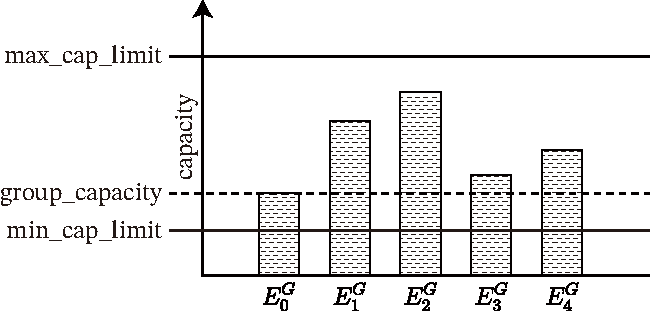
\includegraphics[width=0.85\linewidth]{fig/capacities_in_group}}
	\caption{Example of Capacity of Links Belonging to a Group and the Group Capacity}
	\label{fig:capacities_in_group}
\end{figure}

\subsection{Group Construction}

\subsubsection{Link Recruitment}

For group construction, we assume sufficient links exist in the PCN for grouping. All PC participants can act as group constructors, defining lower limit \mincaplimit{} and upper limit \maxcaplimit{} for link capacities in their group, along with the number of links \groupsize{} needed to establish the group, broadcasting \groupreq{} messages at regular intervals.

When receiving \groupreq{} messages from other nodes, if a node has links satisfying the capacity conditions, it compares the sender's node ID with its own (treating both as integers). To avoid group overlap, it responds only if the sender's ID is larger and stops its own group construction. When a constructor receives \groupsize{} responses to \groupreq{} messages, it finalizes the group links and simultaneously sends group capacity calculation requests \groupcapreq{} with unique \texttt{group\_update\_id} to all source nodes of group links.

\subsubsection{Group Capacity Calculation}

For a group $G$ consisting of $k$ links, the procedure for finding only the minimum capacity (group capacity) among group links without directly sharing individual link capacities is as follows. Source nodes $V_{i}^{G}(i=0,1,\ldots,k-1)$ of links $E_{i}^{G}(i=0,1,\ldots,k-1)$ belonging to group $G$ each independently wait a random time after receiving the group capacity calculation request, then send \groupcap{} messages containing their link's actual capacity, a unique random value $r_{i}$, and \texttt{group\_update\_id} to the next indexed node $V_{j}^{G}$ where $j=(i+1)\bmod k$.

Upon receiving this, node $V_{j}^{G}$ overwrites the value if link $E_{j}^{G}$'s capacity is smaller than the received value and forwards the \groupcap{} message to node $V_{(j+1)\bmod k}^{G}$. Among the $k$ times node $V_{j}^{G}$ receives the same \groupcap{} message, it forwards without updating the value for randomly selected $\lfloor \frac{k}{2} \rfloor$ times.

When node $V_{i}^{G}$ receives a \groupcap{} message containing its unique random value $r_{i}$, it considers this contains the minimum capacity value updated by all group links and broadcasts this value along with \texttt{group\_update\_id} as a \groupupdate{} message. All PCN nodes collect $k$ \groupupdate{} messages with the same \texttt{group\_update\_id} and consider the most frequently appearing value as group $G$'s group capacity, updating their locally maintained PCN topology information.

The group capacity obtained this way makes it difficult for third parties to identify which link actually has the minimum value, making it hard to track capacity changes to specific links. This makes estimating payment amounts and parties for specific links difficult, maintaining payment information confidentiality.

\begin{figure}[htbp]
	\centerline{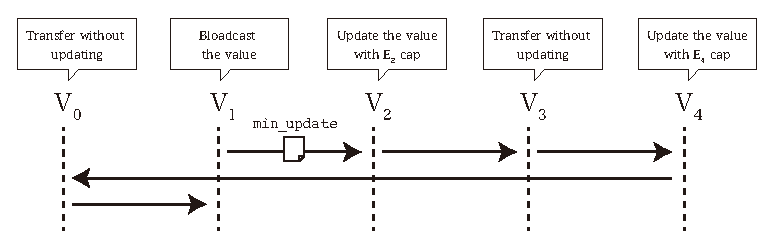
\includegraphics[width=1\linewidth]{fig/group_cap_handover}}
	\caption{Example of \groupcap{} Message Propagation}
	\label{fig:group_cap_sequence}
\end{figure}

\subsection{Payment Using Group Capacity Information}

When group capacity is broadcast, senders estimate capacity for each link as follows:
\begin{itemize}
	\item If a link belongs to some group: use that group's capacity as the link's capacity
	\item If not in any group: use the publicly disclosed channel capacity as link capacity
\end{itemize}

When senders perform actual route exploration, they search for minimum-cost routes similar to Lightning Network~\cite{poon_dryja_2016,lnd,eclair,clightning}, but use the above values as link capacities. That is, senders use only links whose estimated capacity exceeds the payment amount and select the minimum-cost route.

Upon successful payment, group capacity update requests are simultaneously sent to all groups containing route links, updating group capacity to the latest state through procedures similar to the group capacity calculation.

\subsection{Group Capacity Update}

When payments are executed, capacities of links on the payment route change. Therefore, senders simultaneously send group capacity update requests to all member nodes of groups containing route links, causing them to recalculate group capacity similar to the group capacity calculation procedure.

Although upstream nodes of capacity-changed links could directly initiate group capacity updates, if the relevant link had the minimum capacity in the group, it could be associated with the minimum value and observed. To avoid this, our method has senders simultaneously request all group members, ensuring all nodes start update processing independently and simultaneously.

When group capacity updates cause values to exceed initially set \mincaplimit{} or \maxcaplimit{}, the group is closed. Upon closure confirmation, \groupupdate{} messages containing invalid group capacity are broadcast to notify group closure. Upstream nodes of closed group links form new groups through the link recruitment procedure.

\section{Performance Evaluation}

This section evaluates how GCB method group construction parameters affect performance and examines parameters that balance payment information confidentiality with payment performance.

\subsection{Evaluation Method}

\subsubsection{Parameters}

Group construction parameters are:
\begin{itemize}
	\item \groupsize{}: Number of links in a group
	\item $\alpha$: Parameter determining group capacity conditions \mincaplimit{} and \maxcaplimit{} where $0 < \alpha < 1$
\end{itemize}

When the group constructor's initial link registered in the group is $E_{const}$ with capacity $cap(E_{const})$, group capacity conditions \mincaplimit{} and \maxcaplimit{} are set using parameter $\alpha (0 < \alpha < 1)$ as:
\begin{align}
	\mincaplimit & = cap(E_{const}) \times (1-\alpha) \\
	\maxcaplimit & = cap(E_{const}) \times (1+\alpha)
\end{align}

\subsubsection{Evaluation Metrics}

Main evaluation metrics are:
\begin{itemize}
	\item Success Rate: Ratio of successful payments to all attempted payments
	\item Latency (Success): Average delay time until successful payment confirmation [ms]
	\item Latency (Fail): Average delay time until failed payment confirmation [ms]
	\item Fail Before Send Rate (FBSR): Probability of detecting no viable route before sending and failing without retries
	\item Fail After Send Rate (FASR): Probability of discovering no viable route after sending and failing after multiple retries
	\item Coverage: Ratio of links belonging to groups to all PCN links
	\item CUL: Link capacity loss rate due to group membership
\end{itemize}

\subsubsection{Simulation Conditions}

We extended the payment channel network simulator CLoTH~\cite{CONOSCENTI2021100717}, which accurately reproduces Lightning Network HTLCs, implementing the GCB method along with two comparison methods:
\begin{itemize}
	\item LN method: Lightning Network method using \channelupdate{} for probabilistic payment route determination
	\item RBB method: Real-time Balance Broadcast (complete disclosure of all link capacities without privacy consideration)
\end{itemize}

We used a Lightning Network snapshot from December 17, 2020, with 6005 nodes and 60913 links. This data was obtained from LND's \texttt{describegraph} command, containing all publicly available information identical to the actual network. Since initial PC balances are undisclosed, we set them using uniformly distributed random numbers. We performed 5000 payments with amounts following normal distribution (mean $\mu = 10000$ sats, variance $\sigma = \mu \times 0.1$) and uniformly distributed random sender/recipient selection.

\subsection{Privacy Evaluation}

We simulated attacks where malicious nodes $V_{m}^{G}$ in groups record all received \groupcap{} messages and randomly select target link $E_{i}^{G}$ capacities to estimate payment amounts, senders, and recipients from capacity changes. Results show that attack success rates decrease with larger \groupsize{}, particularly dropping below 1\% when $\groupsize > 5$, making payment information identification extremely difficult, as shown in Fig.~\ref{fig:group_size_vs_attack_resistance}.

\begin{figure}[htbp]
	\centerline{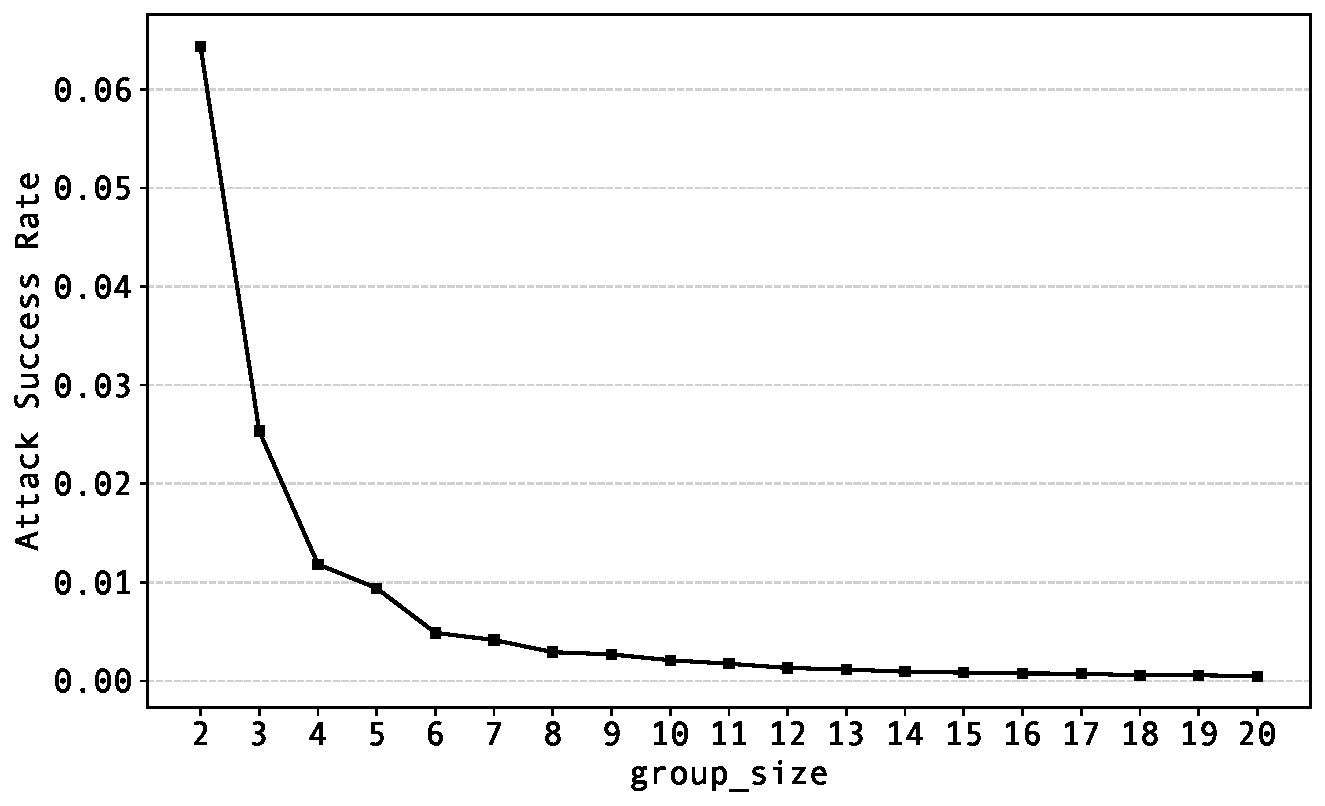
\includegraphics[width=\linewidth]{fig/group_size_vs_attack_resistance}}
	\caption{Variation of Attack Success Rate with respect to \groupsize{}}
	\label{fig:group_size_vs_attack_resistance}
\end{figure}

\subsection{Performance Parameter Evaluation}

We define appropriate parameter regions as those where success rate decrease compared to RBB method is less than 0.005 and FASR increase is less than 0.005. In this region (success rate > 0.729 and FASR < 0.005), maximum average confirmation delay for successful payments was 648 ms at $\groupsize=4, \alpha=0.05$, nearly identical to retry-free RBB method. Maximum average confirmation delay for failed payments was 8.87 ms at $\groupsize=10, \alpha=0.1$, sufficiently smaller than LN method.

This occurs because grouping enables senders to know reliably sendable amounts on group links, allowing exclusion of links with insufficient capacity before route specification, reducing FASR and retry counts to nearly zero.

Based on privacy and performance considerations, we identify $\groupsize=10, \alpha=0.1$ as optimal parameters balancing high success rates with short confirmation delays while maximizing attack resistance. The performance characteristics with varying \groupsize{} and $\alpha$ are shown in Fig.~\ref{fig:group_params_vs_success_rate}.

\begin{figure*}[htbp]
	\centering
	\begin{subfigure}{0.248\textwidth}
		\centering
		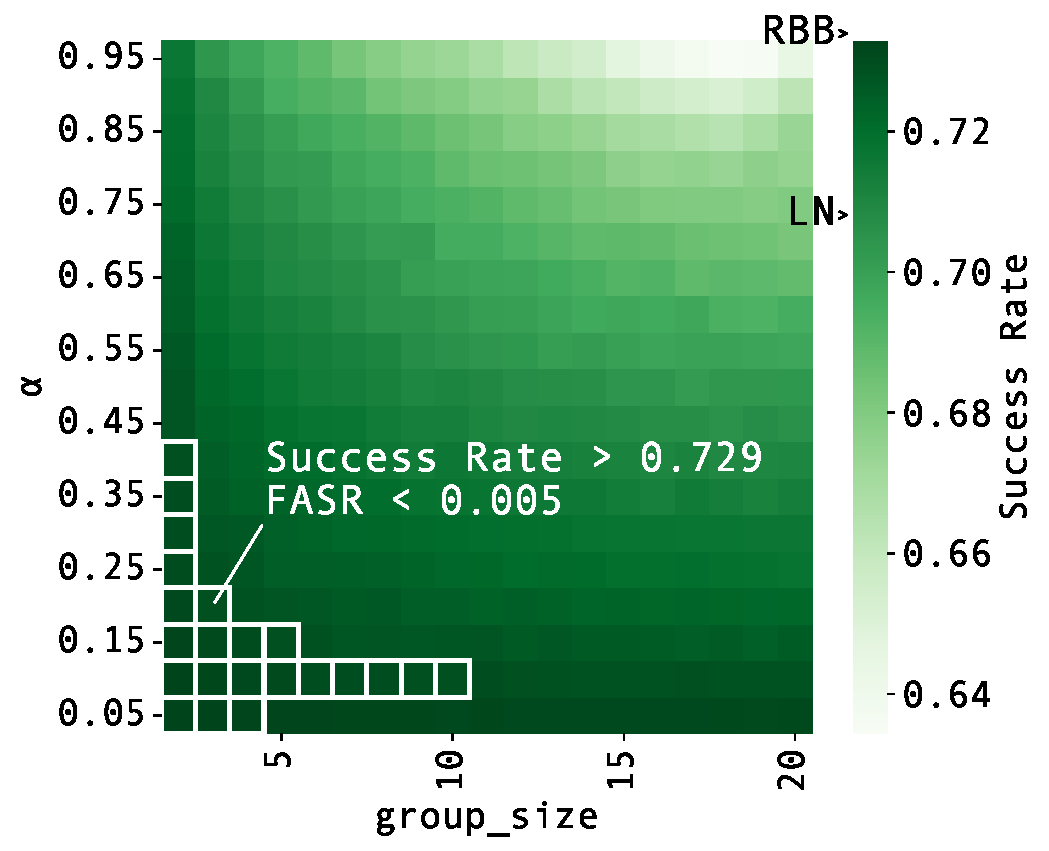
\includegraphics[width=\linewidth]{fig/group_limit_rate_and_group_size_heatmap_success_rate}
		\caption{Success Rate}
	\end{subfigure}
	\hfill
	\begin{subfigure}{0.254\textwidth}
		\centering
		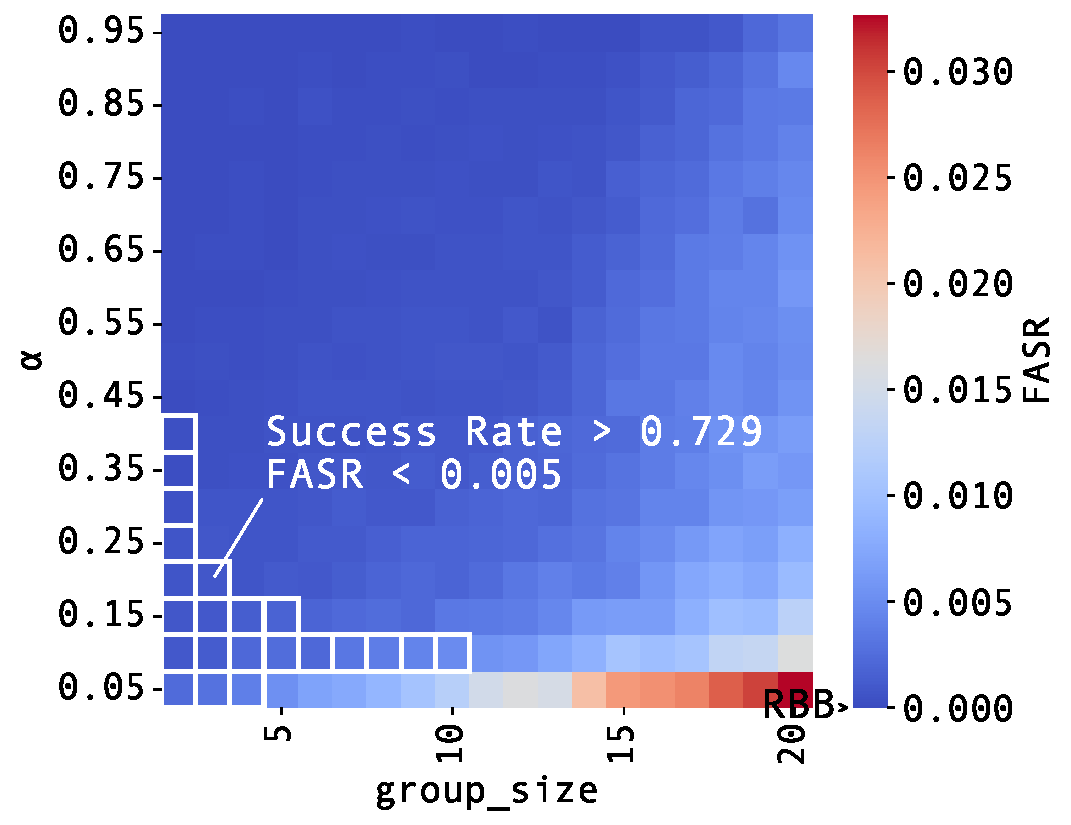
\includegraphics[width=\linewidth]{fig/group_limit_rate_and_group_size_heatmap_fail_after_send_rate}
		\caption{Fail After Send Rate (FASR)}
	\end{subfigure}
	\hfill
	\begin{subfigure}{0.243\textwidth}
		\centering
		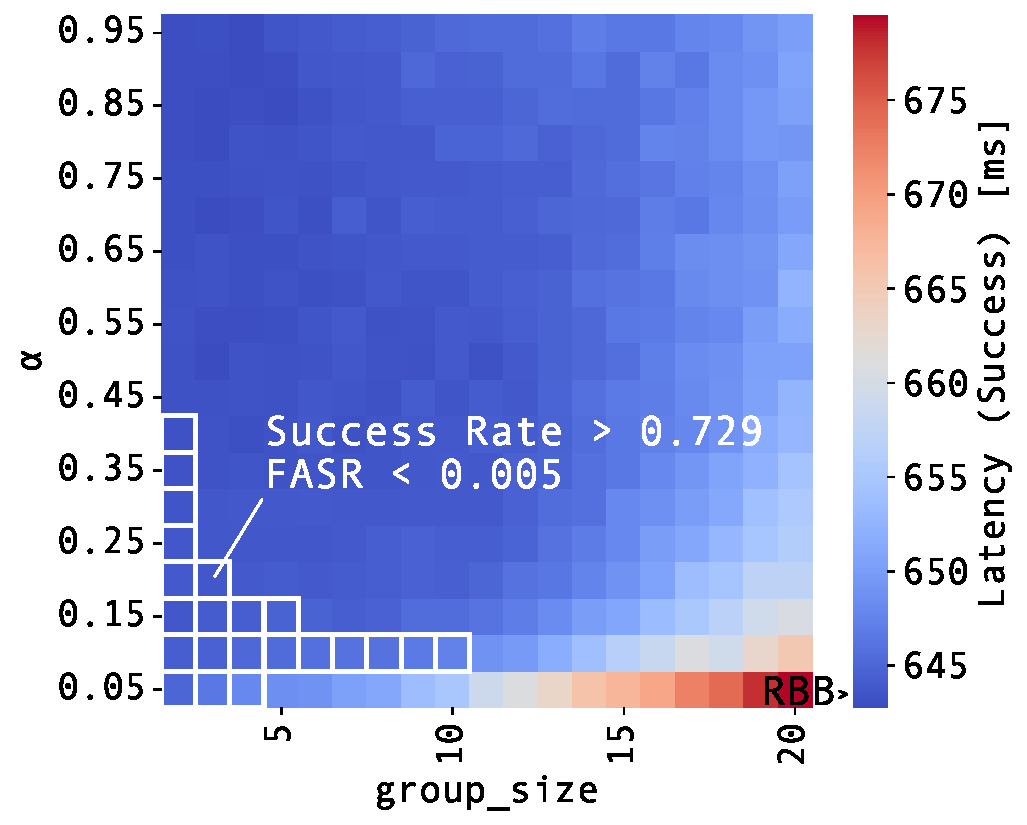
\includegraphics[width=\linewidth]{fig/group_limit_rate_and_group_size_heatmap_latency_success}
		\caption{Latency (Success) [ms]}
	\end{subfigure}
	\hfill
	\begin{subfigure}{0.2375\textwidth}
		\centering
		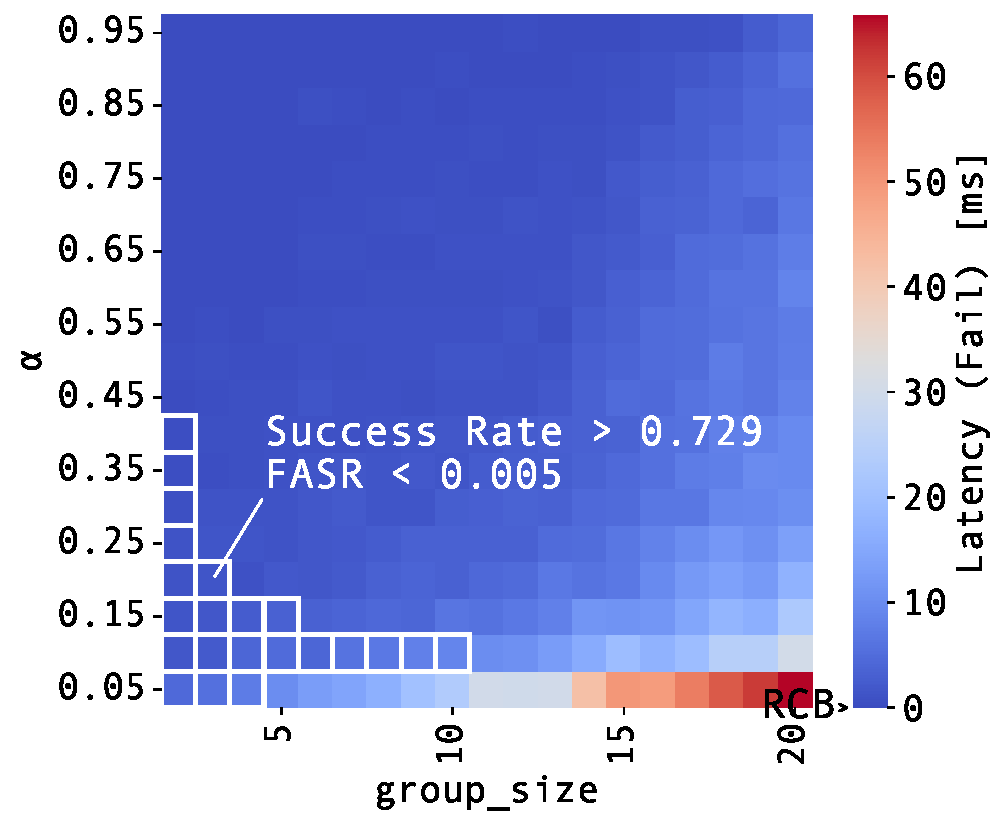
\includegraphics[width=\linewidth]{fig/group_limit_rate_and_group_size_heatmap_latency_fail}
		\caption{Latency (Fail) [ms]}
	\end{subfigure}
	\caption{Performance metrics with varying \groupsize{} and $\alpha$}
	\label{fig:group_params_vs_success_rate}
\end{figure*}

\begin{table}[htbp]
	\caption{Success Rate, FASR and Latency of LN and RBB}
	\centering
	\label{tab:result_group_and_ideal}
	\begin{tabular}{r|cccc}
		    & Success Rate & FASR  & Latency (Success) [ms] & Latency (Fail) [ms] \\
		\hline
		LN  & 0.708        & 0.160 & 826                    & 415                 \\
		RBB & 0.734        & 0.000 & 643                    & 0.000               \\
	\end{tabular}
\end{table}

\subsection{Latency Evaluation}

Using optimal parameters $\groupsize=10, \alpha=0.1$, we compared GCB and LN methods for varying average payment amounts. Results show that while LN method confirmation delays increase significantly with payment amount, GCB method delays increase relatively little. For large payments, LN method experiences many retries due to considering only failure frequency without link capacity, prolonging confirmation time. GCB method eliminates unnecessary retries by disclosing group capacity, enabling immediate pre-send determination of impossible payments and minimizing confirmation delay increases even for large amounts, as demonstrated in Fig.~\ref{fig:pmt_amt_vs_time}.

\begin{figure}[htbp]
	\centerline{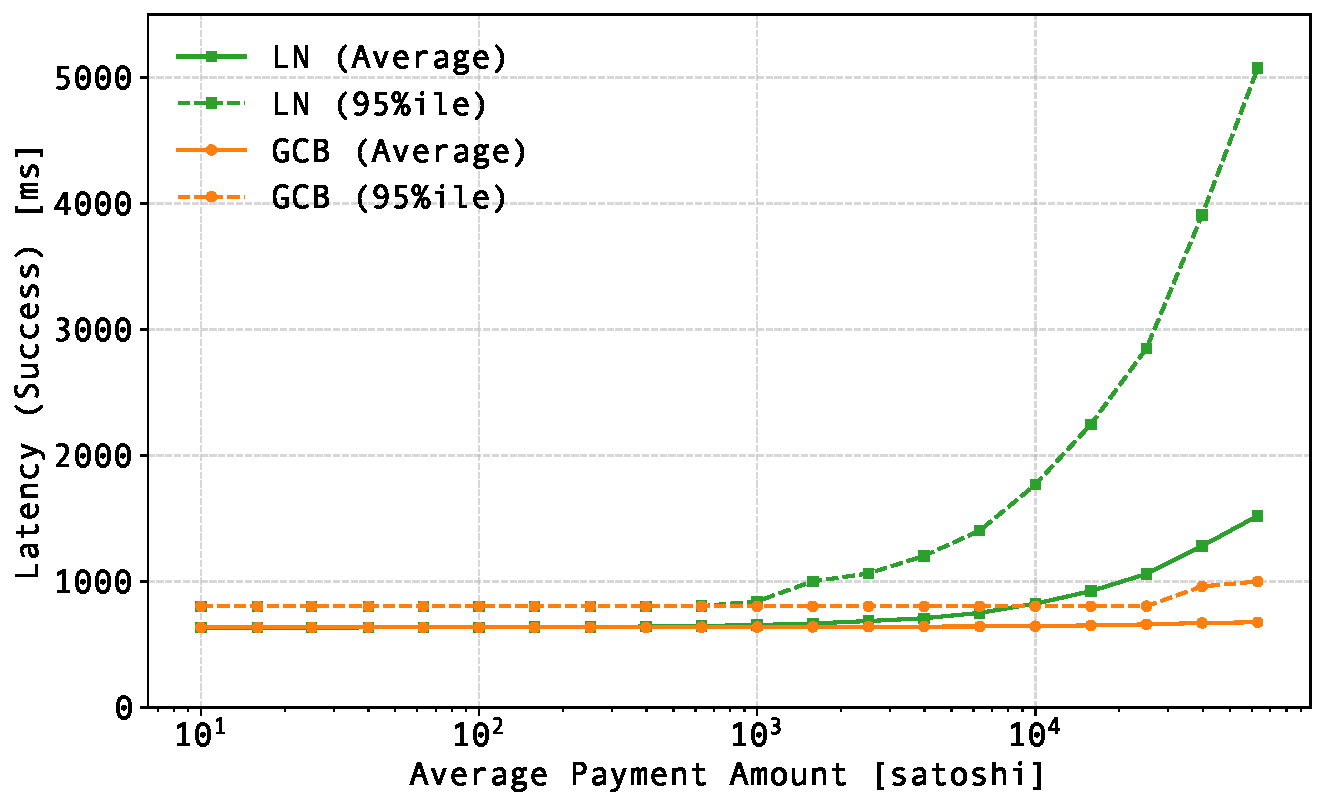
\includegraphics[width=\linewidth]{fig/pmt_amt_vs_time}}
	\caption{Latency of Sending Payment vs Payment Amount for Successful Cases Only}
	\label{fig:pmt_amt_vs_time}
\end{figure}

\section{Conclusion}

This paper presented new evaluations of the GCB method, which groups links in Payment Channel Networks and broadcasts minimum link capacities in real-time as group capacity, maintaining payment information confidentiality while preserving success rates comparable to conventional methods and reducing confirmation delays for successful payments. We identified appropriate values for group capacity and group size parameters. Future work includes verifying payment information confidentiality under more diverse attack models.

\begin{thebibliography}{00}
	\bibitem{nakamoto2008bitcoin} S. Nakamoto, ``Bitcoin: A peer-to-peer electronic cash system,'' 2008.
	\bibitem{poon_dryja_2016} J. Poon and T. Dryja, ``The bitcoin lightning network: Scalable off-chain instant payments,'' 2016.
	\bibitem{lnbolt} ``BOLT: Basis of Lightning Technology,'' \url{https://github.com/lightningnetwork/lightning-rfc}.
	\bibitem{lnd} ``Lightning Network Daemon,'' \url{https://github.com/lightningnetwork/lnd}.
	\bibitem{clightning} ``Core Lightning,'' \url{https://github.com/ElementsProject/lightning}.
	\bibitem{eclair} ``Eclair,'' \url{https://github.com/ACINQ/eclair}.
	\bibitem{Andreescu_2021} O. Andreescu et al., ``Optimizing payment routing in the lightning network,'' in Proc. IEEE INFOCOM, 2021.
	\bibitem{published_papers/48227240} K. Sato and H. Morino, ``Group capacity broadcast method for payment channel networks,'' Technical Report, 2023.
	\bibitem{CONOSCENTI2021100717} M. Conoscenti et al., ``CLoTH: A simulator for HTLC payment networks,'' Future Generation Computer Systems, vol. 118, pp. 1--17, 2021.
\end{thebibliography}

\end{document}
